\documentclass{standalone}
\usepackage{tikz}
\usetikzlibrary{patterns, positioning}
\usepackage[sfdefault]{ClearSans} %% option 'sfdefault' activates Clear Sans as the default text font
\usepackage[T1]{fontenc}

\begin{document}
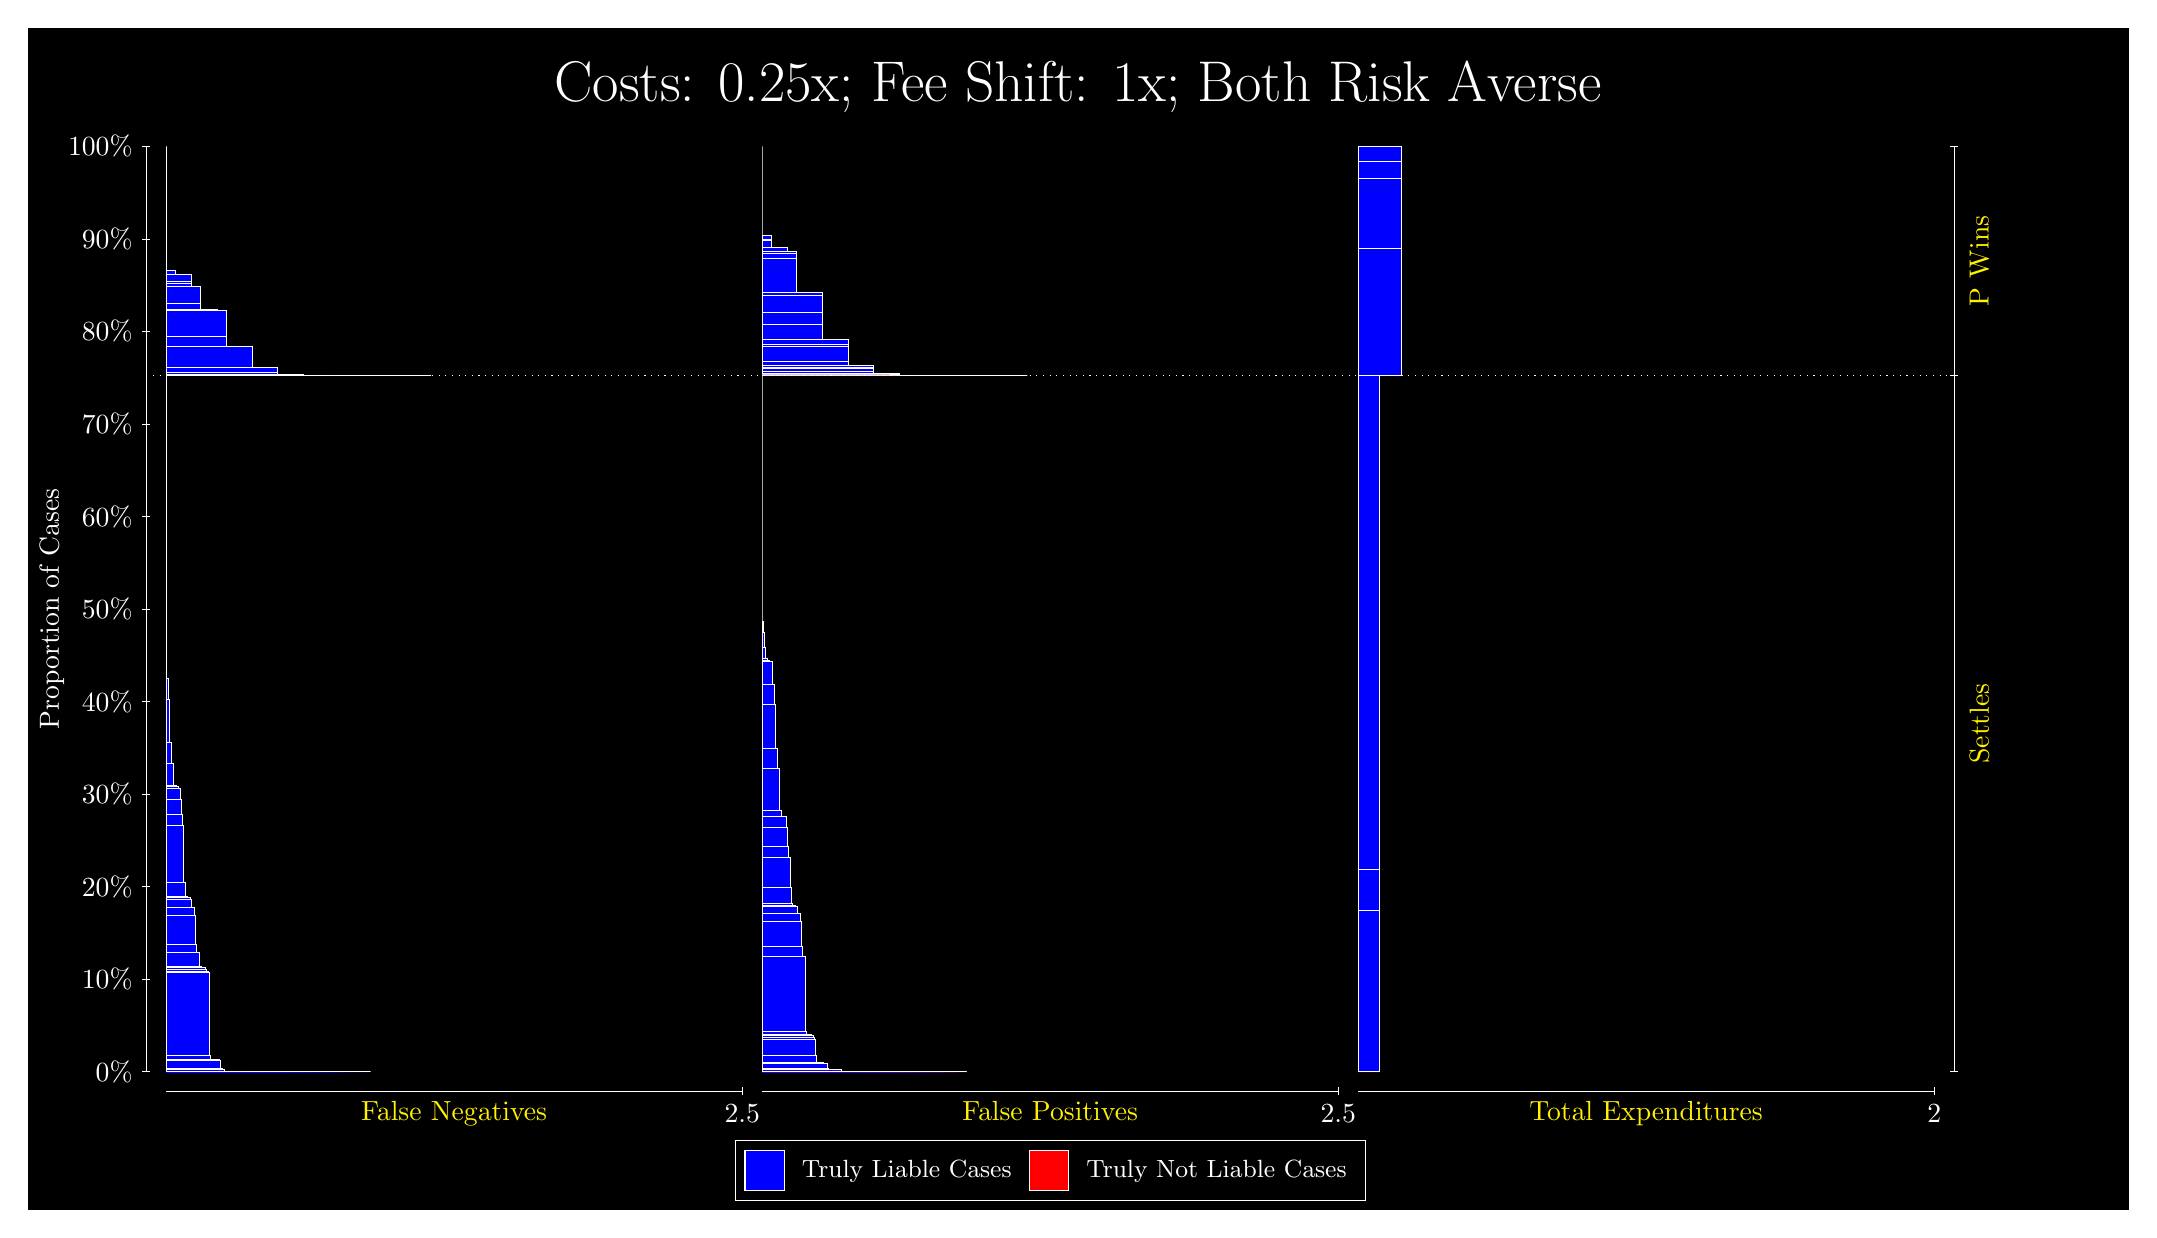
\begin{tikzpicture}
\draw[fill=black] (0,0) rectangle (26.667,15);
\draw[text=white] (0,13.5) rectangle (26.667,15) node[midway] {\huge Costs: 0.25x; Fee Shift: 1x; Both Risk Averse};
\draw[white, very thin] (1.5,1.75) -- (1.5,13.5);
\node[rotate=90, text=white, anchor=center] at (0.3, 7.625) {Proportion of Cases};
\draw[white, very thin] (1.45,1.75) -- (1.55,1.75);
\node[text=white, anchor=east] at (1.45, 1.75) {0\%};
\draw[white, very thin] (1.45,2.925) -- (1.55,2.925);
\node[text=white, anchor=east] at (1.45, 2.925) {10\%};
\draw[white, very thin] (1.45,4.1) -- (1.55,4.1);
\node[text=white, anchor=east] at (1.45, 4.1) {20\%};
\draw[white, very thin] (1.45,5.275) -- (1.55,5.275);
\node[text=white, anchor=east] at (1.45, 5.275) {30\%};
\draw[white, very thin] (1.45,6.45) -- (1.55,6.45);
\node[text=white, anchor=east] at (1.45, 6.45) {40\%};
\draw[white, very thin] (1.45,7.625) -- (1.55,7.625);
\node[text=white, anchor=east] at (1.45, 7.625) {50\%};
\draw[white, very thin] (1.45,8.8) -- (1.55,8.8);
\node[text=white, anchor=east] at (1.45, 8.8) {60\%};
\draw[white, very thin] (1.45,9.975) -- (1.55,9.975);
\node[text=white, anchor=east] at (1.45, 9.975) {70\%};
\draw[white, very thin] (1.45,11.15) -- (1.55,11.15);
\node[text=white, anchor=east] at (1.45, 11.15) {80\%};
\draw[white, very thin] (1.45,12.325) -- (1.55,12.325);
\node[text=white, anchor=east] at (1.45, 12.325) {90\%};
\draw[white, very thin] (1.45,13.5) -- (1.55,13.5);
\node[text=white, anchor=east] at (1.45, 13.5) {100\%};

\draw[white, very thin] (24.457,1.75) -- (24.457,13.5);
\draw[white, very thin] (24.407,1.75) -- (24.507,1.75);
\node[anchor=west] at (24.407, 1.75) {};
\draw[white, very thin] (24.407,10.591) -- (24.507,10.591);
\node[anchor=west] at (24.407, 10.591) {};
\draw[white, very thin] (24.407,13.5) -- (24.507,13.5);
\node[anchor=west] at (24.407, 13.5) {};

\draw[white, very thin, fill=blue] (1.75,1.75) rectangle (4.3482,1.75);
\draw[white, very thin, fill=blue] (1.75,1.75) rectangle (4.2018,1.75);
\draw[white, very thin, fill=blue] (1.75,1.75) rectangle (4.0554,1.75);
\draw[white, very thin, fill=blue] (1.75,1.75) rectangle (4.0229,1.75);
\draw[white, very thin, fill=blue] (1.75,1.75) rectangle (3.9091,1.75);
\draw[white, very thin, fill=blue] (1.75,1.75) rectangle (3.8765,1.75);
\draw[white, very thin, fill=blue] (1.75,1.75) rectangle (3.7627,1.75);
\draw[white, very thin, fill=blue] (1.75,1.75) rectangle (3.7302,1.75);
\draw[white, very thin, fill=blue] (1.75,1.75) rectangle (3.6976,1.75);
\draw[white, very thin, fill=blue] (1.75,1.75) rectangle (3.6163,1.75);
\draw[white, very thin, fill=blue] (1.75,1.75) rectangle (3.5838,1.75);
\draw[white, very thin, fill=blue] (1.75,1.75) rectangle (3.5513,1.75);
\draw[white, very thin, fill=blue] (1.75,1.75) rectangle (3.4699,1.75);
\draw[white, very thin, fill=blue] (1.75,1.75) rectangle (3.4374,1.75);
\draw[white, very thin, fill=blue] (1.75,1.75) rectangle (3.4049,1.75);
\draw[white, very thin, fill=blue] (1.75,1.75) rectangle (3.3723,1.75);
\draw[white, very thin, fill=blue] (1.75,1.75) rectangle (3.3236,1.75);
\draw[white, very thin, fill=blue] (1.75,1.75) rectangle (3.291,1.75);
\draw[white, very thin, fill=blue] (1.75,1.75) rectangle (3.2585,1.75);
\draw[white, very thin, fill=blue] (1.75,1.75) rectangle (3.226,1.75);
\draw[white, very thin, fill=blue] (1.75,1.75) rectangle (3.1772,1.75);
\draw[white, very thin, fill=blue] (1.75,1.75) rectangle (3.1447,1.75);
\draw[white, very thin, fill=blue] (1.75,1.75) rectangle (3.1121,1.75);
\draw[white, very thin, fill=blue] (1.75,1.75) rectangle (3.0796,1.75);
\draw[white, very thin, fill=blue] (1.75,1.75) rectangle (3.0471,1.75);
\draw[white, very thin, fill=blue] (1.75,1.75) rectangle (3.0308,1.75);
\draw[white, very thin, fill=blue] (1.75,1.75) rectangle (2.9983,1.75);
\draw[white, very thin, fill=blue] (1.75,1.75) rectangle (2.9657,1.75);
\draw[white, very thin, fill=blue] (1.75,1.75) rectangle (2.9332,1.75);
\draw[white, very thin, fill=blue] (1.75,1.75) rectangle (2.9007,1.75);
\draw[white, very thin, fill=blue] (1.75,1.75) rectangle (2.8844,1.75);
\draw[white, very thin, fill=blue] (1.75,1.75) rectangle (2.8519,1.75);
\draw[white, very thin, fill=blue] (1.75,1.75) rectangle (2.8194,1.7505);
\draw[white, very thin, fill=blue] (1.75,1.7505) rectangle (2.7868,1.7506);
\draw[white, very thin, fill=blue] (1.75,1.7506) rectangle (2.7543,1.7507);
\draw[white, very thin, fill=blue] (1.75,1.7507) rectangle (2.7218,1.7507);
\draw[white, very thin, fill=blue] (1.75,1.7507) rectangle (2.7055,1.7508);
\draw[white, very thin, fill=blue] (1.75,1.7508) rectangle (2.673,1.7508);
\draw[white, very thin, fill=blue] (1.75,1.7508) rectangle (2.6405,1.7529);
\draw[white, very thin, fill=blue] (1.75,1.7529) rectangle (2.6079,1.7535);
\draw[white, very thin, fill=blue] (1.75,1.7535) rectangle (2.5917,1.7545);
\draw[white, very thin, fill=blue] (1.75,1.7545) rectangle (2.5754,1.7549);
\draw[white, very thin, fill=blue] (1.75,1.7549) rectangle (2.5591,1.7552);
\draw[white, very thin, fill=blue] (1.75,1.7552) rectangle (2.5266,1.7552);
\draw[white, very thin, fill=blue] (1.75,1.7552) rectangle (2.4941,1.7768);
\draw[white, very thin, fill=blue] (1.75,1.7768) rectangle (2.4616,1.7855);
\draw[white, very thin, fill=blue] (1.75,1.7855) rectangle (2.4453,1.898);
\draw[white, very thin, fill=blue] (1.75,1.898) rectangle (2.429,1.9041);
\draw[white, very thin, fill=blue] (1.75,1.9041) rectangle (2.3965,1.9093);
\draw[white, very thin, fill=blue] (1.75,1.9093) rectangle (2.3802,1.9112);
\draw[white, very thin, fill=blue] (1.75,1.9112) rectangle (2.3477,1.9113);
\draw[white, very thin, fill=blue] (1.75,1.9113) rectangle (2.3152,1.9558);
\draw[white, very thin, fill=blue] (1.75,1.9558) rectangle (2.2989,3.0077);
\draw[white, very thin, fill=blue] (1.75,3.0077) rectangle (2.2827,3.0295);
\draw[white, very thin, fill=blue] (1.75,3.0295) rectangle (2.2664,3.0547);
\draw[white, very thin, fill=blue] (1.75,3.0547) rectangle (2.2501,3.0736);
\draw[white, very thin, fill=blue] (1.75,3.0736) rectangle (2.2339,3.0785);
\draw[white, very thin, fill=blue] (1.75,3.0785) rectangle (2.2013,3.0813);
\draw[white, very thin, fill=blue] (1.75,3.0813) rectangle (2.1688,3.2587);
\draw[white, very thin, fill=blue] (1.75,3.2587) rectangle (2.1363,3.3719);
\draw[white, very thin, fill=blue] (1.75,3.3719) rectangle (2.12,3.7323);
\draw[white, very thin, fill=blue] (1.75,3.7323) rectangle (2.1037,3.831);
\draw[white, very thin, fill=blue] (1.75,3.831) rectangle (2.0712,3.9397);
\draw[white, very thin, fill=blue] (1.75,3.9397) rectangle (2.055,3.9691);
\draw[white, very thin, fill=blue] (1.75,3.9691) rectangle (2.0224,3.9709);
\draw[white, very thin, fill=blue] (1.75,3.9709) rectangle (1.9899,4.1483);
\draw[white, very thin, fill=blue] (1.75,4.1483) rectangle (1.9736,4.8785);
\draw[white, very thin, fill=blue] (1.75,4.8785) rectangle (1.9574,5.011);
\draw[white, very thin, fill=blue] (1.75,5.011) rectangle (1.9411,5.2081);
\draw[white, very thin, fill=blue] (1.75,5.2081) rectangle (1.9248,5.3458);
\draw[white, very thin, fill=blue] (1.75,5.3458) rectangle (1.9086,5.3678);
\draw[white, very thin, fill=blue] (1.75,5.3678) rectangle (1.876,5.3854);
\draw[white, very thin, fill=blue] (1.75,5.3854) rectangle (1.8435,5.6669);
\draw[white, very thin, fill=blue] (1.75,5.6669) rectangle (1.811,5.9252);
\draw[white, very thin, fill=blue] (1.75,5.9252) rectangle (1.7947,6.4839);
\draw[white, very thin, fill=blue] (1.75,6.4839) rectangle (1.7785,6.7453);
\draw[white, very thin, fill=red] (1.75,6.7453) rectangle (1.75,6.7453);
\draw[white, very thin, fill=blue] (1.75,6.7453) rectangle (1.75,10.591);
\draw[white, very thin, fill=blue] (1.75,10.591) rectangle (5.1167,10.591);
\draw[white, very thin, fill=blue] (1.75,10.591) rectangle (4.7914,10.591);
\draw[white, very thin, fill=blue] (1.75,10.591) rectangle (4.7914,10.591);
\draw[white, very thin, fill=blue] (1.75,10.591) rectangle (4.4661,10.591);
\draw[white, very thin, fill=blue] (1.75,10.591) rectangle (4.4661,10.591);
\draw[white, very thin, fill=blue] (1.75,10.591) rectangle (4.1408,10.591);
\draw[white, very thin, fill=blue] (1.75,10.591) rectangle (4.027,10.591);
\draw[white, very thin, fill=blue] (1.75,10.591) rectangle (3.8155,10.592);
\draw[white, very thin, fill=blue] (1.75,10.592) rectangle (3.8155,10.592);
\draw[white, very thin, fill=blue] (1.75,10.592) rectangle (3.7017,10.592);
\draw[white, very thin, fill=blue] (1.75,10.592) rectangle (3.7017,10.592);
\draw[white, very thin, fill=blue] (1.75,10.592) rectangle (3.4903,10.607);
\draw[white, very thin, fill=blue] (1.75,10.607) rectangle (3.3764,10.607);
\draw[white, very thin, fill=blue] (1.75,10.607) rectangle (3.165,10.636);
\draw[white, very thin, fill=blue] (1.75,10.636) rectangle (3.165,10.688);
\draw[white, very thin, fill=blue] (1.75,10.688) rectangle (3.0511,10.688);
\draw[white, very thin, fill=blue] (1.75,10.688) rectangle (3.0511,10.688);
\draw[white, very thin, fill=blue] (1.75,10.688) rectangle (2.8397,10.96);
\draw[white, very thin, fill=blue] (1.75,10.96) rectangle (2.7258,10.96);
\draw[white, very thin, fill=blue] (1.75,10.96) rectangle (2.7258,10.96);
\draw[white, very thin, fill=blue] (1.75,10.96) rectangle (2.7258,10.96);
\draw[white, very thin, fill=blue] (1.75,10.96) rectangle (2.5144,11.087);
\draw[white, very thin, fill=blue] (1.75,11.087) rectangle (2.5144,11.42);
\draw[white, very thin, fill=blue] (1.75,11.42) rectangle (2.4006,11.421);
\draw[white, very thin, fill=blue] (1.75,11.421) rectangle (2.4006,11.434);
\draw[white, very thin, fill=blue] (1.75,11.434) rectangle (2.1891,11.502);
\draw[white, very thin, fill=blue] (1.75,11.502) rectangle (2.1891,11.719);
\draw[white, very thin, fill=blue] (1.75,11.719) rectangle (2.0753,11.756);
\draw[white, very thin, fill=blue] (1.75,11.756) rectangle (2.0753,11.787);
\draw[white, very thin, fill=blue] (1.75,11.787) rectangle (2.0753,11.874);
\draw[white, very thin, fill=blue] (1.75,11.874) rectangle (1.8638,11.874);
\draw[white, very thin, fill=blue] (1.75,11.874) rectangle (1.8638,11.879);
\draw[white, very thin, fill=blue] (1.75,11.879) rectangle (1.8638,11.923);
\draw[white, very thin, fill=blue] (1.75,11.923) rectangle (1.8638,11.923);
\draw[white, very thin, fill=red] (1.75,11.923) rectangle (1.75,11.923);
\draw[white, very thin, fill=blue] (1.75,11.923) rectangle (1.75,13.5);
\draw[white, very thin, fill=red] (9.3189,1.75) rectangle (11.917,1.75);
\draw[white, very thin, fill=blue] (9.3189,1.75) rectangle (11.917,1.75);
\draw[white, very thin, fill=red] (9.3189,1.75) rectangle (11.771,1.75);
\draw[white, very thin, fill=blue] (9.3189,1.75) rectangle (11.771,1.75);
\draw[white, very thin, fill=red] (9.3189,1.75) rectangle (11.624,1.75);
\draw[white, very thin, fill=blue] (9.3189,1.75) rectangle (11.624,1.75);
\draw[white, very thin, fill=blue] (9.3189,1.75) rectangle (11.592,1.75);
\draw[white, very thin, fill=blue] (9.3189,1.75) rectangle (11.445,1.75);
\draw[white, very thin, fill=red] (9.3189,1.75) rectangle (11.332,1.75);
\draw[white, very thin, fill=blue] (9.3189,1.75) rectangle (11.332,1.75);
\draw[white, very thin, fill=blue] (9.3189,1.75) rectangle (11.299,1.75);
\draw[white, very thin, fill=blue] (9.3189,1.75) rectangle (11.266,1.75);
\draw[white, very thin, fill=red] (9.3189,1.75) rectangle (11.185,1.75);
\draw[white, very thin, fill=blue] (9.3189,1.75) rectangle (11.185,1.75);
\draw[white, very thin, fill=blue] (9.3189,1.75) rectangle (11.12,1.75);
\draw[white, very thin, fill=red] (9.3189,1.75) rectangle (11.039,1.75);
\draw[white, very thin, fill=blue] (9.3189,1.75) rectangle (11.039,1.75);
\draw[white, very thin, fill=blue] (9.3189,1.75) rectangle (11.006,1.75);
\draw[white, very thin, fill=blue] (9.3189,1.75) rectangle (10.974,1.75);
\draw[white, very thin, fill=blue] (9.3189,1.75) rectangle (10.941,1.75);
\draw[white, very thin, fill=red] (9.3189,1.75) rectangle (10.892,1.75);
\draw[white, very thin, fill=blue] (9.3189,1.75) rectangle (10.892,1.75);
\draw[white, very thin, fill=blue] (9.3189,1.75) rectangle (10.86,1.75);
\draw[white, very thin, fill=blue] (9.3189,1.75) rectangle (10.795,1.75);
\draw[white, very thin, fill=red] (9.3189,1.75) rectangle (10.746,1.75);
\draw[white, very thin, fill=blue] (9.3189,1.75) rectangle (10.746,1.75);
\draw[white, very thin, fill=blue] (9.3189,1.75) rectangle (10.714,1.75);
\draw[white, very thin, fill=blue] (9.3189,1.75) rectangle (10.681,1.75);
\draw[white, very thin, fill=blue] (9.3189,1.75) rectangle (10.648,1.7505);
\draw[white, very thin, fill=blue] (9.3189,1.7505) rectangle (10.616,1.7505);
\draw[white, very thin, fill=red] (9.3189,1.7505) rectangle (10.6,1.7505);
\draw[white, very thin, fill=blue] (9.3189,1.7505) rectangle (10.6,1.7505);
\draw[white, very thin, fill=blue] (9.3189,1.7505) rectangle (10.567,1.7505);
\draw[white, very thin, fill=blue] (9.3189,1.7505) rectangle (10.535,1.7505);
\draw[white, very thin, fill=blue] (9.3189,1.7505) rectangle (10.47,1.7528);
\draw[white, very thin, fill=red] (9.3189,1.7528) rectangle (10.453,1.7528);
\draw[white, very thin, fill=blue] (9.3189,1.7528) rectangle (10.453,1.7529);
\draw[white, very thin, fill=blue] (9.3189,1.7529) rectangle (10.421,1.7529);
\draw[white, very thin, fill=blue] (9.3189,1.7529) rectangle (10.388,1.753);
\draw[white, very thin, fill=blue] (9.3189,1.753) rectangle (10.356,1.7531);
\draw[white, very thin, fill=blue] (9.3189,1.7531) rectangle (10.323,1.775);
\draw[white, very thin, fill=red] (9.3189,1.775) rectangle (10.307,1.775);
\draw[white, very thin, fill=blue] (9.3189,1.775) rectangle (10.307,1.7763);
\draw[white, very thin, fill=blue] (9.3189,1.7763) rectangle (10.291,1.7768);
\draw[white, very thin, fill=blue] (9.3189,1.7768) rectangle (10.274,1.7773);
\draw[white, very thin, fill=blue] (9.3189,1.7773) rectangle (10.242,1.7774);
\draw[white, very thin, fill=blue] (9.3189,1.7774) rectangle (10.209,1.7792);
\draw[white, very thin, fill=red] (9.3189,1.7792) rectangle (10.161,1.7792);
\draw[white, very thin, fill=blue] (9.3189,1.7792) rectangle (10.161,1.7974);
\draw[white, very thin, fill=blue] (9.3189,1.7974) rectangle (10.144,1.8512);
\draw[white, very thin, fill=blue] (9.3189,1.8512) rectangle (10.128,1.8581);
\draw[white, very thin, fill=blue] (9.3189,1.8581) rectangle (10.095,1.863);
\draw[white, very thin, fill=blue] (9.3189,1.863) rectangle (10.063,1.8658);
\draw[white, very thin, fill=blue] (9.3189,1.8658) rectangle (10.03,1.8686);
\draw[white, very thin, fill=red] (9.3189,1.8686) rectangle (10.014,1.8686);
\draw[white, very thin, fill=blue] (9.3189,1.8686) rectangle (10.014,1.9616);
\draw[white, very thin, fill=blue] (9.3189,1.9616) rectangle (9.9979,2.1562);
\draw[white, very thin, fill=blue] (9.3189,2.1562) rectangle (9.9816,2.1812);
\draw[white, very thin, fill=blue] (9.3189,2.1812) rectangle (9.9654,2.2054);
\draw[white, very thin, fill=blue] (9.3189,2.2054) rectangle (9.9491,2.2245);
\draw[white, very thin, fill=blue] (9.3189,2.2245) rectangle (9.9166,2.2262);
\draw[white, very thin, fill=blue] (9.3189,2.2262) rectangle (9.884,2.2552);
\draw[white, very thin, fill=red] (9.3189,2.2552) rectangle (9.8678,2.2552);
\draw[white, very thin, fill=blue] (9.3189,2.2552) rectangle (9.8678,3.2142);
\draw[white, very thin, fill=blue] (9.3189,3.2142) rectangle (9.8353,3.3441);
\draw[white, very thin, fill=blue] (9.3189,3.3441) rectangle (9.819,3.6581);
\draw[white, very thin, fill=blue] (9.3189,3.6581) rectangle (9.8027,3.7579);
\draw[white, very thin, fill=blue] (9.3189,3.7579) rectangle (9.7702,3.8443);
\draw[white, very thin, fill=blue] (9.3189,3.8443) rectangle (9.7377,3.862);
\draw[white, very thin, fill=blue] (9.3189,3.862) rectangle (9.7051,3.8809);
\draw[white, very thin, fill=blue] (9.3189,3.8809) rectangle (9.6889,4.0847);
\draw[white, very thin, fill=blue] (9.3189,4.0847) rectangle (9.6726,4.4747);
\draw[white, very thin, fill=blue] (9.3189,4.4747) rectangle (9.6563,4.6087);
\draw[white, very thin, fill=blue] (9.3189,4.6087) rectangle (9.6401,4.8552);
\draw[white, very thin, fill=blue] (9.3189,4.8552) rectangle (9.6238,4.9913);
\draw[white, very thin, fill=blue] (9.3189,4.9913) rectangle (9.5913,4.9957);
\draw[white, very thin, fill=blue] (9.3189,4.9957) rectangle (9.5588,5.0691);
\draw[white, very thin, fill=blue] (9.3189,5.0691) rectangle (9.5425,5.5956);
\draw[white, very thin, fill=blue] (9.3189,5.5956) rectangle (9.51,5.857);
\draw[white, very thin, fill=blue] (9.3189,5.857) rectangle (9.4937,6.4156);
\draw[white, very thin, fill=blue] (9.3189,6.4156) rectangle (9.4774,6.6739);
\draw[white, very thin, fill=blue] (9.3189,6.6739) rectangle (9.4449,6.9554);
\draw[white, very thin, fill=blue] (9.3189,6.9554) rectangle (9.4124,6.9731);
\draw[white, very thin, fill=blue] (9.3189,6.9731) rectangle (9.3799,6.9951);
\draw[white, very thin, fill=blue] (9.3189,6.9951) rectangle (9.3636,7.1328);
\draw[white, very thin, fill=blue] (9.3189,7.1328) rectangle (9.3473,7.3299);
\draw[white, very thin, fill=blue] (9.3189,7.3299) rectangle (9.3311,7.4623);
\draw[white, very thin, fill=blue] (9.3189,7.4623) rectangle (9.3189,10.591);
\draw[white, very thin, fill=red] (9.3189,10.591) rectangle (12.686,10.591);
\draw[white, very thin, fill=blue] (9.3189,10.591) rectangle (12.686,10.591);
\draw[white, very thin, fill=red] (9.3189,10.591) rectangle (12.36,10.591);
\draw[white, very thin, fill=blue] (9.3189,10.591) rectangle (12.36,10.591);
\draw[white, very thin, fill=red] (9.3189,10.591) rectangle (12.035,10.591);
\draw[white, very thin, fill=blue] (9.3189,10.591) rectangle (12.035,10.591);
\draw[white, very thin, fill=blue] (9.3189,10.591) rectangle (12.035,10.591);
\draw[white, very thin, fill=blue] (9.3189,10.591) rectangle (12.035,10.591);
\draw[white, very thin, fill=red] (9.3189,10.591) rectangle (11.71,10.591);
\draw[white, very thin, fill=blue] (9.3189,10.591) rectangle (11.71,10.591);
\draw[white, very thin, fill=blue] (9.3189,10.591) rectangle (11.71,10.591);
\draw[white, very thin, fill=red] (9.3189,10.591) rectangle (11.384,10.591);
\draw[white, very thin, fill=blue] (9.3189,10.591) rectangle (11.384,10.592);
\draw[white, very thin, fill=blue] (9.3189,10.592) rectangle (11.384,10.593);
\draw[white, very thin, fill=red] (9.3189,10.593) rectangle (11.271,10.593);
\draw[white, very thin, fill=blue] (9.3189,10.593) rectangle (11.271,10.593);
\draw[white, very thin, fill=blue] (9.3189,10.593) rectangle (11.059,10.6);
\draw[white, very thin, fill=red] (9.3189,10.6) rectangle (11.059,10.6);
\draw[white, very thin, fill=blue] (9.3189,10.6) rectangle (11.059,10.605);
\draw[white, very thin, fill=blue] (9.3189,10.605) rectangle (11.059,10.614);
\draw[white, very thin, fill=red] (9.3189,10.614) rectangle (10.945,10.614);
\draw[white, very thin, fill=blue] (9.3189,10.614) rectangle (10.945,10.614);
\draw[white, very thin, fill=blue] (9.3189,10.614) rectangle (10.734,10.649);
\draw[white, very thin, fill=blue] (9.3189,10.649) rectangle (10.734,10.679);
\draw[white, very thin, fill=red] (9.3189,10.679) rectangle (10.734,10.679);
\draw[white, very thin, fill=blue] (9.3189,10.679) rectangle (10.734,10.699);
\draw[white, very thin, fill=blue] (9.3189,10.699) rectangle (10.734,10.721);
\draw[white, very thin, fill=blue] (9.3189,10.721) rectangle (10.62,10.721);
\draw[white, very thin, fill=red] (9.3189,10.721) rectangle (10.62,10.721);
\draw[white, very thin, fill=blue] (9.3189,10.721) rectangle (10.62,10.721);
\draw[white, very thin, fill=blue] (9.3189,10.721) rectangle (10.409,10.769);
\draw[white, very thin, fill=red] (9.3189,10.769) rectangle (10.409,10.769);
\draw[white, very thin, fill=blue] (9.3189,10.769) rectangle (10.409,10.955);
\draw[white, very thin, fill=blue] (9.3189,10.955) rectangle (10.409,10.992);
\draw[white, very thin, fill=blue] (9.3189,10.992) rectangle (10.409,11.053);
\draw[white, very thin, fill=blue] (9.3189,11.053) rectangle (10.295,11.053);
\draw[white, very thin, fill=red] (9.3189,11.053) rectangle (10.295,11.053);
\draw[white, very thin, fill=blue] (9.3189,11.053) rectangle (10.295,11.053);
\draw[white, very thin, fill=blue] (9.3189,11.053) rectangle (10.083,11.236);
\draw[white, very thin, fill=blue] (9.3189,11.236) rectangle (10.083,11.388);
\draw[white, very thin, fill=blue] (9.3189,11.388) rectangle (10.083,11.612);
\draw[white, very thin, fill=blue] (9.3189,11.612) rectangle (10.083,11.648);
\draw[white, very thin, fill=blue] (9.3189,11.648) rectangle (9.9694,11.648);
\draw[white, very thin, fill=red] (9.3189,11.648) rectangle (9.9694,11.648);
\draw[white, very thin, fill=blue] (9.3189,11.648) rectangle (9.9694,11.649);
\draw[white, very thin, fill=blue] (9.3189,11.649) rectangle (9.758,12.074);
\draw[white, very thin, fill=blue] (9.3189,12.074) rectangle (9.758,12.145);
\draw[white, very thin, fill=blue] (9.3189,12.145) rectangle (9.758,12.167);
\draw[white, very thin, fill=blue] (9.3189,12.167) rectangle (9.6442,12.167);
\draw[white, very thin, fill=red] (9.3189,12.167) rectangle (9.6442,12.167);
\draw[white, very thin, fill=blue] (9.3189,12.167) rectangle (9.6442,12.217);
\draw[white, very thin, fill=blue] (9.3189,12.217) rectangle (9.6442,12.217);
\draw[white, very thin, fill=blue] (9.3189,12.217) rectangle (9.4327,12.304);
\draw[white, very thin, fill=blue] (9.3189,12.304) rectangle (9.4327,12.32);
\draw[white, very thin, fill=blue] (9.3189,12.32) rectangle (9.4327,12.368);
\draw[white, very thin, fill=blue] (9.3189,12.368) rectangle (9.4327,12.371);
\draw[white, very thin, fill=red] (9.3189,12.371) rectangle (9.3189,12.371);
\draw[white, very thin, fill=blue] (9.3189,12.371) rectangle (9.3189,13.5);
\draw[white, very thin, fill=red] (16.888,1.75) rectangle (17.162,1.75);
\draw[white, very thin, fill=blue] (16.888,1.75) rectangle (17.162,3.8032);
\draw[white, very thin, fill=red] (16.888,3.8032) rectangle (17.162,3.8032);
\draw[white, very thin, fill=blue] (16.888,3.8032) rectangle (17.162,4.3176);
\draw[white, very thin, fill=red] (16.888,4.3176) rectangle (17.162,4.3176);
\draw[white, very thin, fill=blue] (16.888,4.3176) rectangle (17.162,10.591);
\draw[white, very thin, fill=red] (16.888,10.591) rectangle (17.437,10.591);
\draw[white, very thin, fill=blue] (16.888,10.591) rectangle (17.437,12.209);
\draw[white, very thin, fill=red] (16.888,12.209) rectangle (17.437,12.209);
\draw[white, very thin, fill=blue] (16.888,12.209) rectangle (17.437,13.099);
\draw[white, very thin, fill=red] (16.888,13.099) rectangle (17.437,13.099);
\draw[white, very thin, fill=blue] (16.888,13.099) rectangle (17.437,13.316);
\draw[white, very thin, fill=red] (16.888,13.316) rectangle (17.437,13.316);
\draw[white, very thin, fill=blue] (16.888,13.316) rectangle (17.437,13.5);
\draw[white, dotted] (1.5,10.591) -- (24.457,10.591);
\draw[white, very thin] (1.75,1.5) -- (9.0689,1.5);
\node[text=yellow, anchor=north] at (5.4094, 1.5) {False Negatives};
\draw[white, very thin] (9.0689,1.45) -- (9.0689,1.55);
\node[text=white, anchor=north] at (9.0689, 1.45) {2.5};

\draw[white, very thin] (9.3189,1.5) -- (16.638,1.5);
\node[text=yellow, anchor=north] at (12.978, 1.5) {False Positives};
\draw[white, very thin] (16.638,1.45) -- (16.638,1.55);
\node[text=white, anchor=north] at (16.638, 1.45) {2.5};

\draw[white, very thin] (16.888,1.5) -- (24.207,1.5);
\node[text=yellow, anchor=north] at (20.547, 1.5) {Total Expenditures};
\draw[white, very thin] (24.207,1.45) -- (24.207,1.55);
\node[text=white, anchor=north] at (24.207, 1.45) {2};

\node[text=yellow, centered, rotate=90] at (24.777, 6.1704) {Settles};
\node[text=yellow, centered, rotate=90] at (24.777, 12.045) {P Wins};

\draw (12.978300999999998,1.5) node[draw=none] (baseCoordinate) {};
\begin{scope}[align=center]
        \matrix[scale=0.5, draw=white, below=0.5cm of baseCoordinate, nodes={draw}, column sep=0.1cm]{
            \node[rectangle, draw, minimum width=0.5cm, minimum height=0.5cm, fill=blue] {}; &
            \node[draw=none, font=\small, text=white] (B) {Truly Liable Cases}; &
            \node[rectangle, draw, minimum width=0.5cm, minimum height=0.5cm, fill=red] {}; &
            \node[draw=none, font=\small, text=white] (B) {Truly Not Liable Cases}; \\
            };
\end{scope}

\end{tikzpicture}
\end{document}